% CS631 Advanced Programming in the UNIX Environment
% Author: Jan Schaumann <jschauma@netmeister.org>
% $Id: slides.tex,v 1.2 2005/11/01 16:41:35 jschauma Exp $
\special{! TeXDict begin /landplus90{true}store end }

\documentclass[xga]{xdvislides}
\usepackage[landscape]{geometry}
\usepackage{graphics}
\usepackage{graphicx}
\usepackage{colordvi}
\usepackage{xcolor}

\begin{document}
\setfontphv

%%% Headers and footers
\lhead{\slidetitle}
\chead{CS631 - Advanced Programming in the UNIX Environment}
\rhead{Slide \thepage}
\lfoot{\Gray{Lecture 09: D\ae mon processes, System Logging, Advanced I/O}}
\cfoot{\relax}
\rfoot{\Gray{\today}}

\newcommand{\smallish}{\fontsize{15}{20}\selectfont}

\vspace*{\fill}
\begin{center}
	\Hugesize
		CS631 - Advanced Programming in the UNIX Environment\\
		-- \\
		D\ae mon processes, System Logging, Advanced I/O\\
	\hspace*{5mm}\blueline\\ [1em]
	\Normalsize
		Department of Computer Science\\
		Stevens Institute of Technology\\
		Jan Schaumann\\
		\verb+jschauma@stevens.edu+\\
		\verb+https://www.cs.stevens.edu/~jschauma/631/+
\end{center}
\vspace*{\fill}

\subsection{D\ae mon processes}
So... what's a d\ae mon process anyway?
\vfill
\hfill
\includegraphics[scale=0.5]{pics/daemon.eps} \\

\subsection{D\ae mon characteristics}
Commonly, d\ae mon processes are created to offer a specific service.
\\

D\ae mon processes usually
\begin{itemize}
	\item live for a long time
	\item are started at boot time
	\item terminate only during shutdown
	\item have no controlling terminal
\end{itemize}

\vfill
\hfill
\includegraphics[scale=0.5]{pics/daemon.eps} \\

\subsection{D\ae mon characteristics}
The previously listed characteristics have certain implications:
\\

\begin{itemize}
	\item do one thing, and one thing only
	\item no (or only limited) user-interaction possible
	\item resource leaks eventually surface
	\item consider current working directory
	\item how to create (debugging) output
\end{itemize}

\vfill
\hfill
\includegraphics[scale=0.5]{pics/daemon.eps} \\

\subsection{Writing a d\ae mon}
\begin{itemize}
	\item fork off the parent process
	\item change file mode mask (umask)
	\item create a unique Session ID (SID)
	\item change the current working directory to a safe place
	\item close (or redirect) standard file descriptors
	\item open any logs for writing
	\item enter actual d\ae mon code
\end{itemize}

\vfill
\hfill
\includegraphics[scale=0.5]{pics/daemon.eps} \\

\subsection{Writing a d\ae mon}
\small
\begin{verbatim}
int
daemon(int nochdir, int noclose)
{
        int fd;

        switch (fork()) {
        case -1:
                return (-1);
        case 0:
                break;
        default:
                _exit(0);
        }

        if (setsid() == -1)
                return (-1);

        if (!nochdir)
                (void)chdir("/");

        if (!noclose && (fd = open(_PATH_DEVNULL, O_RDWR, 0)) != -1) {
                (void)dup2(fd, STDIN_FILENO);
                (void)dup2(fd, STDOUT_FILENO);
                (void)dup2(fd, STDERR_FILENO);
                if (fd > STDERR_FILENO)
                        (void)close(fd);
        }
        return (0);
}
\end{verbatim}
\Normalsize

\subsection{D\ae mon conventions}
\begin{itemize}
	\item prevent against multiple instances via a {\em lockfile}
	\item allow for easy determination of PID via a {\em pidfile}
	\item configuration file convention {\tt /etc/{\em name}.conf}
	\item include a system initialization script (for {\tt /etc/rc.d/} or {\tt
		/etc/init.d/})
	\item re-read configuration file upon {\tt SIGHUP}
	\item relay information via {\em event logging}
\end{itemize}

\vfill
\hfill
\includegraphics[scale=0.5]{pics/daemon.eps} \\

\subsection{A central logging facility}

There are three ways to generate log messages:
\begin{itemize}
	\item via the kernel routine {\tt log(9)}
	\item via the userland routine {\tt syslog(3)}
	\item via UDP messages to port 514
\end{itemize}

\subsection{A central logging facility}
\begin{center}
	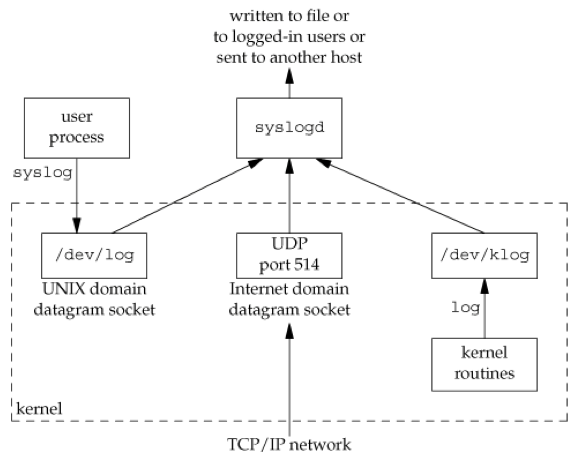
\includegraphics[scale=0.8,angle=-90]{pics/syslog.eps}
\end{center}


\subsection{\tt syslog(3)}
\small
\setlength{\unitlength}{1mm}
\begin{center}
	\begin{picture}(150,22)
		\thinlines
		\put(0,0){\framebox(130,22){}}
		\put(10,17){{\tt \#include <syslog.h>}}
		\put(10,10){{\tt void openlog(const char *{\em ident}, int {\em logopt}, int {\em facility});}}
		\put(10,5){{\tt void syslog(int {\em priority}, const char *{\em message}, ...);}}
	\end{picture}
\end{center}
\Normalsize
{\tt openlog(3)} allows us to set specific options when logging:
\begin{itemize}
	\item prepend {\em ident} to each message
	\item specify logging options ({\tt LOG\_CONS | LOG\_NDELAY | LOG\_PERRO | LOG\_PID})
	\item specify a {\em facility} (such as {\tt LOG\_DAEMON}, {\tt LOG\_MAIL} etc.)
\end{itemize}
\vspace{.5in}
{\tt syslog(3)} writes a message to the system message logger, tagged with
{\em priority}. \\
A {\em priority} is a combination of a {\em facility} (as above) and a {\em level} (such
as {\tt LOG\_DEBUG}, {\tt LOG\_WARNING} or {\tt LOG\_EMERG}).

\subsection{Nonblocking I/O}
Recall from our lecture on signals that certain system calls can block forever:
\begin{itemize}
	\item {\tt read(2)} from a particular file, if data isn't present (pipes,
		terminals, network devices)
	\item {\tt write(2)} to the same kind of file
	\item {\tt open(2)} of a particular file until a specific condition occurs
	\item {\tt read(2)} and {\tt write(2)} of files that have mandatory
		locking enabled
	\item certain {\tt ioctls(2)}
	\item some IPC functions (such as {\tt sendto(2)} or {\tt recv(2)})
\end{itemize}
\vspace{.25in}
See {\tt eintr.c} from that lecture.

\subsection{Nonblocking I/O}
Recall from our lecture on signals that certain system calls can block forever:
\begin{itemize}
	\item {\tt read(2)} from a particular file, if data isn't present (pipes,
		terminals, network devices)
	\item {\tt write(2)} to the same kind of file
	\item {\tt open(2)} of a particular file until a specific condition occurs
	\item {\tt read(2)} and {\tt write(2)} of files that have mandatory
		locking enabled
	\item certain {\tt ioctls(2)}
	\item some IPC functions (such as {\tt sendto(2)} or {\tt recv(2)})
\end{itemize}
\vspace{.25in}
Nonblocking I/O lets us issue an I/O operation and not have it block forever.
If the operation cannot be completed, return is made immediately with an error
noting that the operating would have blocked ({\tt EWOULDBLOCK} or {\tt EAGAIN}).

\subsection{Nonblocking I/O}
Ways to specify nonblocking mode:
\begin{itemize}
	\item pass {\tt O\_NONBLOCK} to {\tt open(2)}: \\

		{\tt open({\em path}, O\_RDRW|O\_NONBLOCK);}
		\vspace{.2in}
	\item set {\tt O\_NONBLOCK} via {\tt fcntl(2)}: \\

		{\tt flags = fcntl({\em fd}, F\_GETFL, 0); \\
		     fcntl({\em fd}, F\_SETFL, flags|O\_NONBLOCK);}
\end{itemize}

\subsection{Nonblocking I/O}
\begin{verbatim}
$ cc -Wall nonblock.c -o block
$ cc -DNONBLOCK -Wall nonblock.c -o nonblock
$ ./nonblock >/dev/null
wrote 100000 bytes
[...]
$ ./block | ( sleep 3; cat >/dev/null )
[...]
$ ./nonblock | ( sleep 3; cat >/dev/null )
[...]
$ ( ./nonblock | cat >/dev/null ) 2>&1 | more
[...]
$ nc -l 8080 >/dev/null &

$ ./nonblock | nc hostname 8080
[...]
\end{verbatim}

\subsection{Resource Locking}
Ways we have learned so far to ensure only one process has exclusive
access to a resource:
\begin{itemize}
	\item open file using {\tt O\_CREAT|O\_EXCL}, then immediately
		{\tt unlink(2)} it
	\item create a ``lockfile'' -- if file exists, somebody else is
		using the resource
	\item use of a semaphore
\end{itemize}

What are some problems with each of these?

\subsection{Advisory Locking}
\small
\setlength{\unitlength}{1mm}
\begin{center}
	\begin{picture}(150,22)
		\thinlines
		\put(0,0){\framebox(130,22){}}
		\put(10,17){{\tt \#include <fcntl.h>}}
		\put(10,10){{\tt int flock(int {\em fd},int {\em operation});}}
		\put(80,3){Returns: 0 if OK, -1 otherwise}
	\end{picture}
\end{center}
\Normalsize
\begin{itemize}
	\item applies or removes an advisory lock on the file associated with
		the file descriptor fd
	\item {\em operation} can be {\tt LOCK\_NB} and any one of:
		\begin{itemize}
			\item {\tt LOCK\_SH}
			\item {\tt LOCK\_EX}
			\item {\tt LOCK\_UN}
		\end{itemize}
	\item locks entire file
\end{itemize}

\subsection{Advisory Locking}
\begin{verbatim}
$ cc -Wall flock.c
1$ ./a.out
Shared lock established - sleeping for 10 seconds.
[...]
Giving up all locks.

2$ ./a.out
Shared lock established - sleeping for 10 seconds.
Now trying to get an exclusive lock.
Unable to get an exclusive lock.
[...]
Exclusive lock established.

1$ ./a.out
[blocks until the other process terminates]


\end{verbatim}

\subsection{Advisory ``Record'' Locking}
Record locking is done using {\tt fcntl(2)}, using one of {\tt F\_GETLK}, {\tt
F\_SETLK} or {\tt F\_SETLKW} and passing a
\begin{verbatim}
struct flock {
    short l_type;   /* F_RDLCK, F_WRLCK, or F_UNLCK */
    off_t l_start;  /* offset in bytes from l_whence */
    short l_whence; /* SEEK_SET, SEEK_CUR, or SEEK_END */
    off_t l_len;    /* length, in bytes; 0 means "lock to EOF" */
    pid_t l_pid;    /* returned by F_GETLK */
}
\end{verbatim}
Lock types are:
\begin{itemize}
	\item {\tt F\_RDLCK} -- Non-exclusive (read) lock; fails if write lock exists.
	\item {\tt F\_WRLCK} -- Exclusive (write) lock; fails if any lock exists.
	\item {\tt F\_UNLCK} -- Releases our lock on specified range.
\end{itemize}


\subsection{Advisory ``Record'' locking}
\small
\setlength{\unitlength}{1mm}
\begin{center}
	\begin{picture}(180,20)
		\thinlines
		\put(0,0){\framebox(160,20){}}
		\put(10,15){{\tt \#include <unistd.h>}}
		\put(10,7){{\tt int lockf(int {\em fd}, int {\em value}, off\_t {\em size});}}
		\put(100,3){Returns: 0 on success, -1 on error}
	\end{picture}
\end{center}
\Normalsize

{\em value} can be:
\begin{itemize}
	\item {\tt F\_ULOCK} -- unlock locked sections
	\item {\tt F\_LOCK} -- lock a section for exclusive use
	\item {\tt F\_TLOCK} -- test and lock a section for exclusive use
	\item {\tt F\_TEST} -- test a section for locks by other processes
\end{itemize}
\begin{center}
	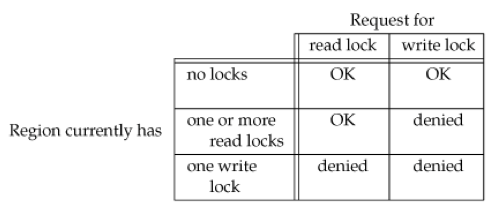
\includegraphics[scale=0.7,angle=-90]{pics/locking.eps}
\end{center}

\subsection{Advisory ``Record'' locking}
Locks are:
\begin{itemize}
	\item released if a process terminates
	\item released if a filedescriptor is closed (!)
	\item not inherited across {\tt fork(2)}
	\item inherited across {\tt exec(2)}
	\item released upon {\tt exec(2)} if close-on-exec is set
\end{itemize}

% \subsection{Advisory ``Record'' locking}
% Locks are associated with a {\em file and process pair}, not with a {\em filedescriptor}!
% \begin{verbatim}
% fd1 = open(pathname, ...);
% write_lock(fd1...);        /* lock byte 0 */
% if ((pid = fork()) > 0) {
%         fd2 = dup(fd1);
%         fd3 = open(pathname, ...);
% } else if (pid == 0) {
%         read_lock(fd1...); /* lock byte 1 */
% }
% \end{verbatim}
%
\subsection{Advisory ``Record'' locking}
Locks are associated with a {\em file and process pair}, not with a {\em filedescriptor}!
\begin{center}
	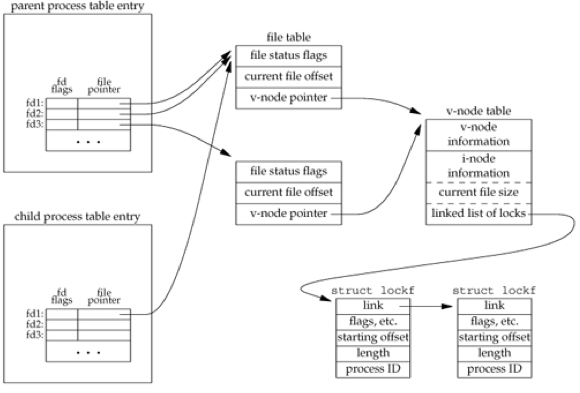
\includegraphics[scale=0.8,angle=-90]{pics/locking-structures.eps}
\end{center}

\subsection{Mandatory locking}
\begin{itemize}
	\item not implemented on all UNIX flavors
		\begin{itemize}
			\item {\tt chmod g+s,g-x file}
		\end{itemize}
	\item possible to be circumvented:
\end{itemize}
\begin{verbatim}
$ mandatory-lock /tmp/file &
$ echo foo > /tmp/file2
$ rm /tmp/file
$ mv /tmp/file2 /tmp/file
\end{verbatim}

\subsection{Asynchronous I/O}
\begin{center}
\includegraphics[scale=1.0,angle=-90]{pics/aio1.eps}
\end{center}

\subsection{Synchronous blocking I/O}
\begin{center}
\includegraphics[scale=1.0,angle=-90]{pics/aio2.eps}
\end{center}

\subsection{Synchronous non-blocking I/O}
\begin{center}
\includegraphics[scale=1.0,angle=-90]{pics/aio3.eps}
\end{center}

\subsection{"Asynchronous" blocking I/O}
\begin{center}
\includegraphics[scale=1.0,angle=-90]{pics/aio4.eps}
\end{center}

\subsection{Asynchronous non-blocking I/O}
\begin{center}
\includegraphics[scale=1.0,angle=-90]{pics/aio5.eps}
\end{center}


\subsection{Asynchronous I/O}
\begin{itemize}
	\item System V derived async I/O
		\begin{itemize}
			\item limited to STREAMS
			\item enabled via {\tt ioctl(2)}
			\item uses {\tt SIGPOLL}
		\end{itemize}
	\item BSD derived async I/O
		\begin{itemize}
			\item limited to terminals and networks
			\item enabled via {\tt fcntl(2)} ({\tt O\_ASYNC},
{\tt  F\_SETOWN})
			\item uses {\tt SIGIO} and {\tt SIGURG}
		\end{itemize}
	\item POSIX \verb+aio(3)+
		\begin{itemize}
			\item kernel process manages queued I/O requests
			\item notification of calling process via signal or \verb+sigevent+ callback function
			\item calling process can still choose to block/wait
		\end{itemize}
\end{itemize}

\subsection{Memory Mapped I/O}
\small
\setlength{\unitlength}{1mm}
\begin{center}
	\begin{picture}(180,30)
		\thinlines
		\put(0,0){\framebox(160,30){}}
		\put(10,25){{\tt \#include <sys/types.h>}}
		\put(10,20){{\tt \#include <sys/mman.h>}}
		\put(10,12){{\tt void *mmap(void *{\em addr}, size\_t {\em len}, int {\em prot}, int {\em flags}, int {\em fd}, off\_t {\em offset});}}
		\put(95,3){Returns: pointer to mapped region if OK}
	\end{picture}
\end{center}
\Normalsize
Protection specified for a region:
\begin{itemize}
	\item {\tt PROT\_READ} -- region can be read
	\item {\tt PROT\_WRITE} -- region can be written
	\item {\tt PROT\_EXEC} -- region can be executed
	\item {\tt PROT\_NONE} -- region can not be accessed
\end{itemize}
\vspace{.25in}
{\em flag} needs to be one of
\begin{itemize}
	\item {\tt MAP\_SHARED}
	\item {\tt MAP\_PRIVATE}
	\item {\tt MAP\_COPY}
\end{itemize}
which may be OR'd with other flags (see {\tt mmap(2)} for details).

\subsection{Memory Mapped I/O}
\begin{center}
	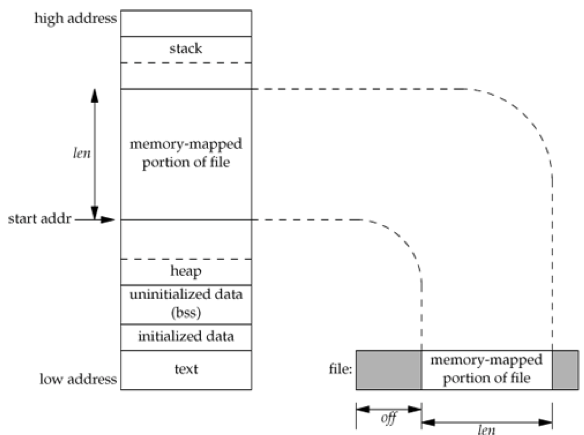
\includegraphics[scale=0.8,angle=-90]{pics/mmap.eps}
\end{center}

\subsection{Memory Mapped I/O}
\begin{center}
	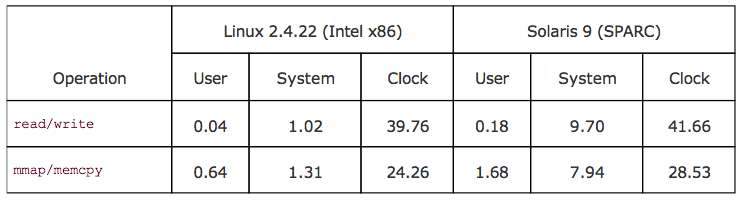
\includegraphics[scale=0.8,angle=-90]{pics/mmap-timing.eps}
\end{center}
\addvspace{.5in}
Exercise: write a program that benchmarks this performance and run it on
the systems you have access to.

\subsection{Memory Mapped I/O}
\\
\vspace*{\fill}
\verb+http://cvsweb.netbsd.org/bsdweb.cgi/src/bin/cp/utils.c?rev=HEAD+
\vspace*{\fill}

\subsection{Reading}
\begin{verbatim}
https://www.ibm.com/developerworks/linux/library/l-async/index.html
http://menehune.opt.wfu.edu/Kokua/More_SGI/007-2478-008/sgi_html/ch08.html
http://lse.sourceforge.net/io/aionotes.txt
https://en.wikipedia.org/wiki/STREAMS
\end{verbatim}

\end{document}
